%\section{Theory}
\section {Early Evidence of the Internal Structure of Nucleon}
\pdfcomment{magnetic moment of proton and neutron}
The first evident of nucleons being a composite particles comes form the 
measurement of their magnetic moment. For spin 1/2 elementary particles, the 
magnetic moment can be expressed as 
\begin{equation}
\mu = \frac{g}{2}\mu_B ~~~~ \mu_B = \frac{e\hbar}{2m},
\end{equation}
with $g$ expected to be $2$. Such measurement was first carried out by Otto 
Stern in 1933. And they found that the $g$ factor for proton is significantly 
greater than $2$. Since the neutron is a neutral particle, it was expected that
to have a zero magnetic moment. Stern and his team would later found that the 
neutron moment to be non-zero, suggesting that proton and neutron are composite
particles.
\pdfcomment{find appropriate citation. The original paper on proton magnetic
	moment is in Germany which I can't read}

\pdfcomment{proton form factor can be determined from e-p elastic scattering,
	which is related to the charge distribution in proton and neutron}
In the 1950s, the proton form factor was measured using electron proton elastic
scattering experiments\cite{hofstadter1956}. The elastic scattering cross 
section can be expressed as 
\begin{equation}
\dv{\sigma}{\Omega} = \left(\dv{\sigma}{\Omega}\right)_{Mott}\left\{ 
	\frac{G_E^2\left(Q^2\right) + \frac{Q^2}{4M^2}G_M^2 \left(Q^2\right)}
	{1 + \frac{Q^2}{4M^2}} + \frac{Q^2}{2M^2} G^2_M{Q^2}\tan^2\frac{\theta}{2}
	\right\},
\end{equation}
where $Q^2$ is the momentum transferred squared, and $G_E\left(Q^2\right)$ is 
known as the electric form factor and can be interpreted as the Fourier 
transform of the charged distribution. The deviation of the neutron electric 
form factor from zero illustrate the existence of internal structures in 
nucleons. Fig.\ \ref{fig:charge} shows the extracted proton and neutron charge 
density from the electric form factor taken from Ref.\ \cite{miller2007}.
\begin{figure}[htbp!]
    \centering
    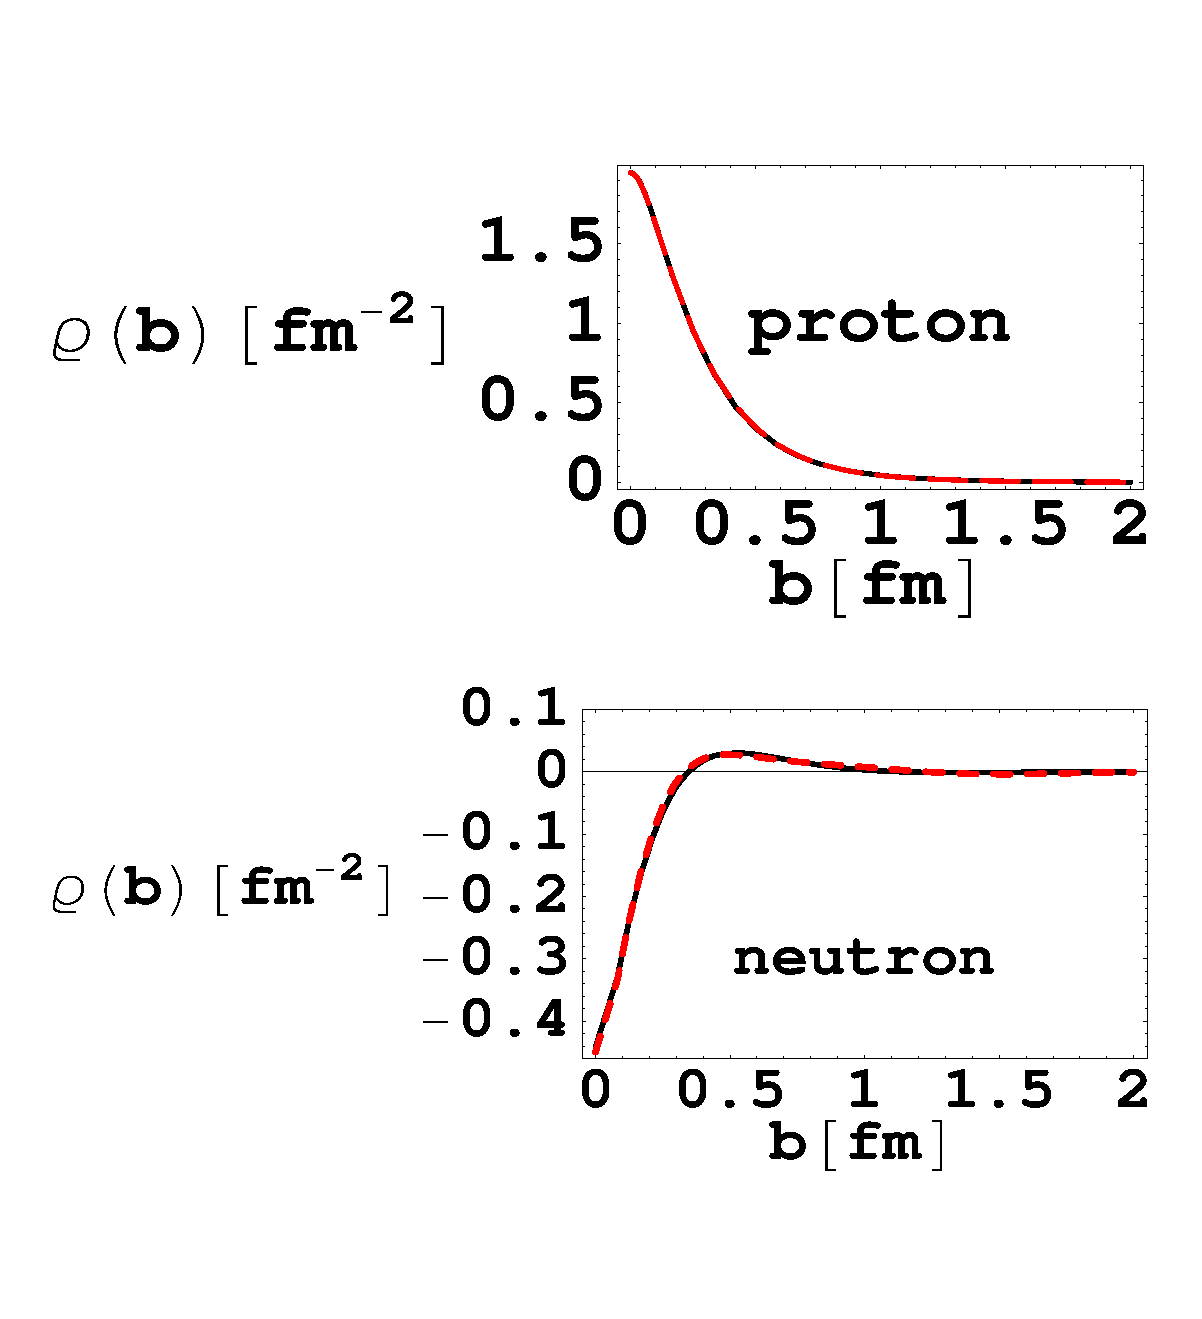
\includegraphics[width=0.5\linewidth]{./images/charge_distribution}
    \caption{The proton charge density (upper panel) and neutron charge density
	(lower panel). Taken from Ref.\ \cite{miller2007}}.
    \label{fig:charge}
\end{figure}


\section {Deep Inelastic Scattering}
\label{sec:dis}
Evidence of the point-like constituents in the nucleon first came from the deep
inelastic scattering (DIS) experiments \cite{breidenbach1969}, where a high 
energy lepton ($l$) is inelastically scattered of a nucleon ($N$), as 
illustrated in Fig.\ \ref{fig:DIS}
\begin{equation}
	l + N \rightarrow l^\prime + X.
\end{equation}
\begin{figure}[htbp!]
    \centering
    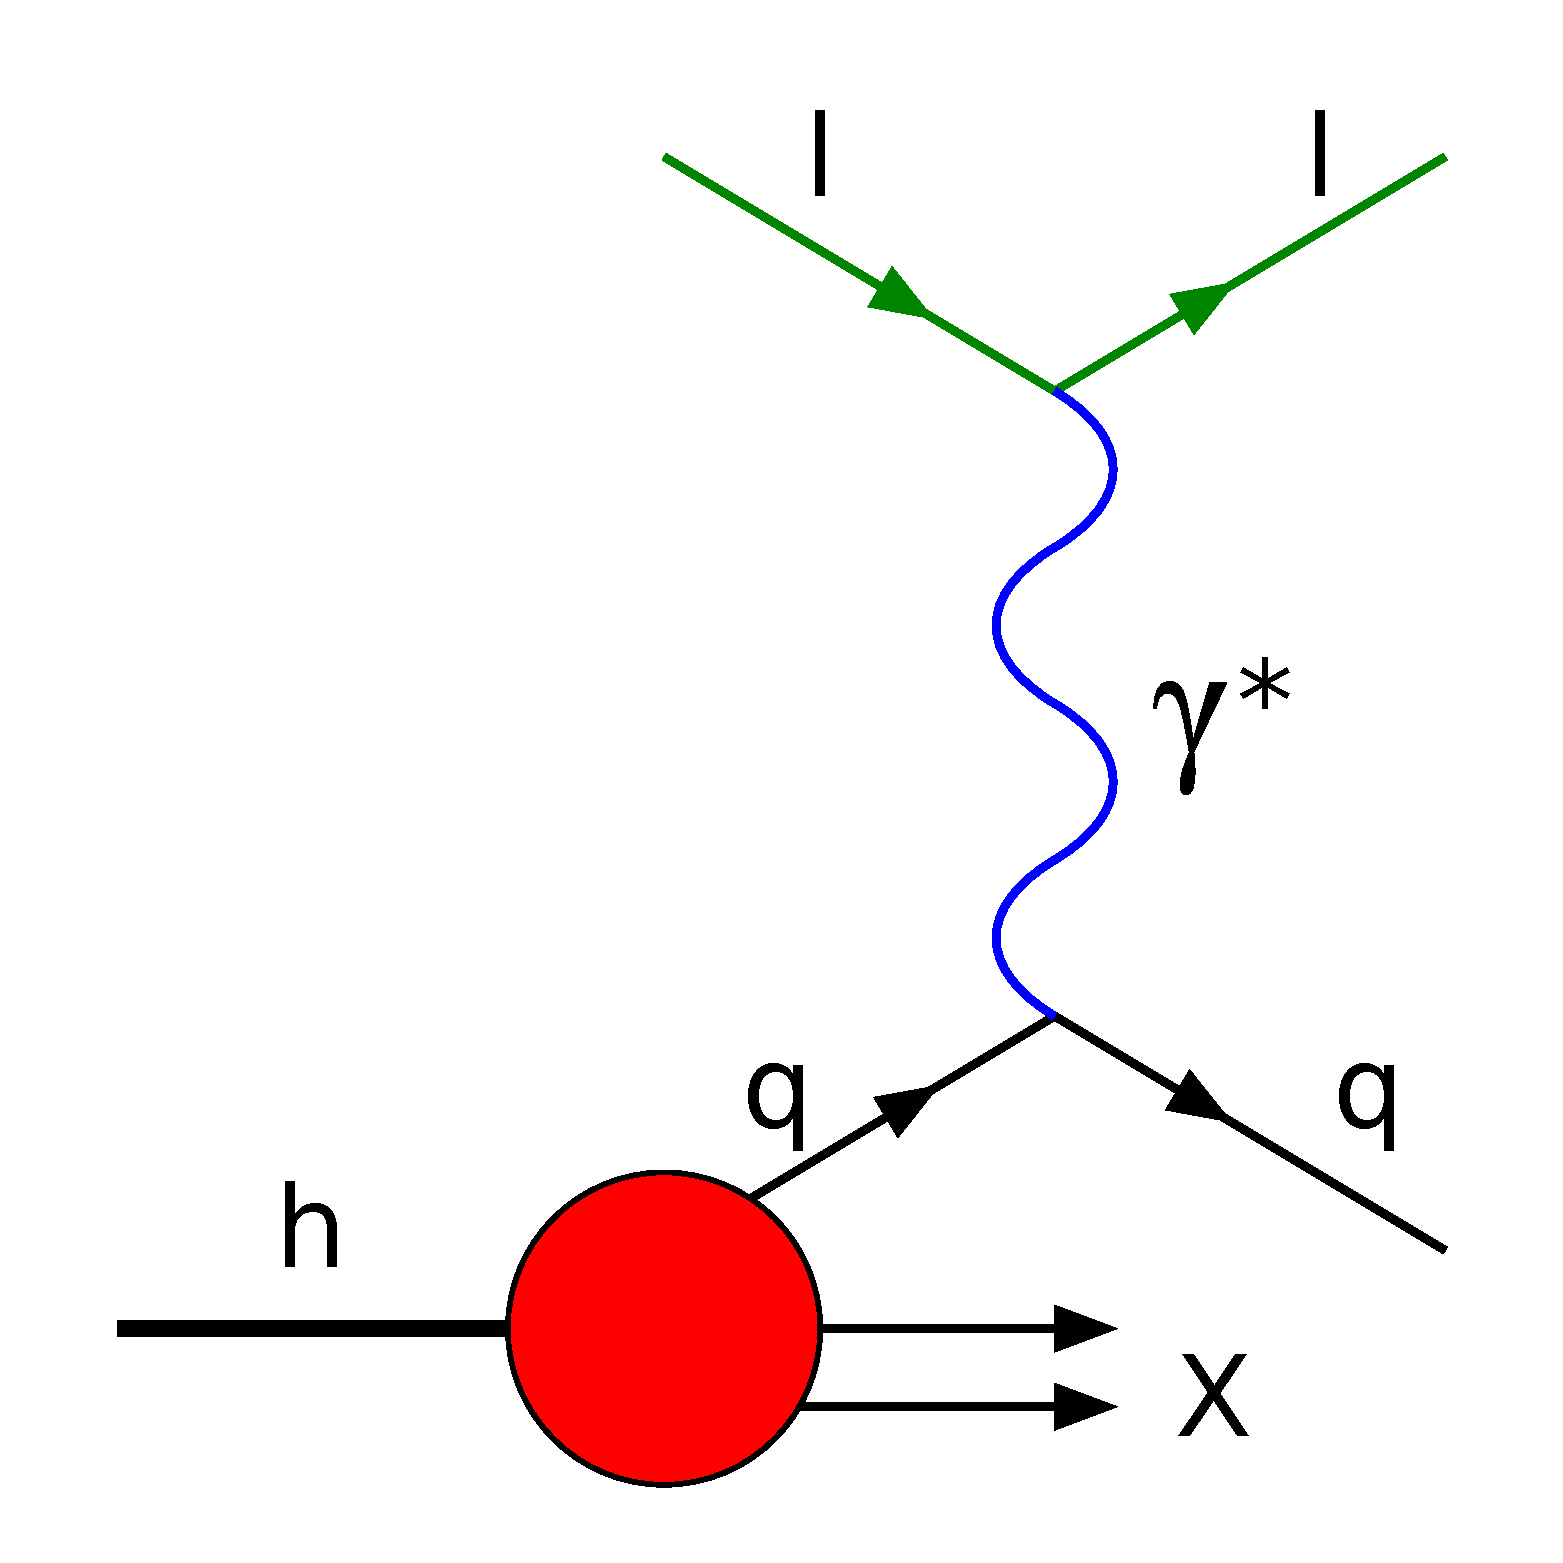
\includegraphics[width=0.5\linewidth]{./images/DIS}
    \caption{The Feynman diagram for DIS}
    \label{fig:DIS}
\end{figure}
The double differential cross section for DIS in the laboratory frame is given 
as
\begin{equation}
	\eval{\pdv{\sigma}{E^\prime}{\Omega}}_{DIS} = \frac{\alpha^2}{4E^2 \sin^4 
	\frac{\theta}{2}} \left[ \frac{1}{\nu}F_2\left(x,Q^2\right)\cos^2
	\frac{\theta}{2} + \frac{1}{M} F_1\left(x,Q^2\right)\sin^2 \frac{\theta}{2}
	\right]
\end{equation}



\pdfcomment{colin-gross relation shows that the protons are made up of spin 1/2
	partons. This relation would be different if the spin of partons is 
	different}


\section{Parton Model}
\label{sec:parton}

\subsection{Gottfried Sum Rule}
\label{sec:gottfried}

\section{Drell-Yan Process}
\label{sec:DY}

\pdfcomment{factorization and universality of PDF, scaling plot for both DIS 
	and DY}

\subsection{E866/NuSea}
\label{sec:E866}

\section{Charmonium Production}
\label{sec:jpsi}
The mechanism for charmonium production can be separated into two parts, the 
production of heavy-quark pairs and the subsequent hadronization into 
quarkonium states. One of the early approaches is the Color Evaporation method 
(CEM)\cite{einhorn1975,bodwin1995,bodwin1997}. The heavy-quark pairs production
is expanded in terms of the strong coupling constant s and is calculated with 
perturbative QCD (pQCD). CEM then assumes a constant probability $F$ for the 
$c\bar{c}$ pairs to hadronize into different charmonium state and this 
probability is independent of the kinematics or the production subprocess. The 
charmonium production cross section in the CEM framework can be expressed as
\begin{equation}
\eval{\dv{\sigma}{x_{F}}}_{J/\psi\left(\psi^\prime\right)} =
	F_{J/\psi\left(\psi^\prime\right)} \sum_{i,j=q,\bar{q},g} \int_{2m_c}^{2m_D}
\end{equation}


\pdfcomment{CEM and NRCD}

\pdfcomment{what is physical significant of the nuclear dependence}

